
\documentclass[12pt]{article}

\usepackage[utf8]{inputenc}
\usepackage[greek, english]{babel}

% Packages
\usepackage{MnSymbol}
\usepackage{alphabeta}
\usepackage{amsfonts}
\usepackage{amsmath}
\usepackage{amsthm}
\usepackage{caption}
\usepackage{graphicx}
\usepackage{latexsym}
\usepackage{stackrel}
\usepackage{titlesec}

% Commands
\newcommand{\R}{\mathbb{R}}
\newcommand{\N}{\mathbb{N}}
\newcommand{\norm}[1]{\left\lVert#1\right\rVert}
\newcommand{\margin}{\hspace{4pt}}
\newcommand{\centered}[1]{\begin{align*}#1\end{align*}}
\newcommand{\plot}{\includegraphics}

% Environments
\newenvironment{rcases}
	{\left.\begin{aligned}}
	{\end{aligned}\right\rbrace}

\newenvironment{matlab}
	{\begin{figure}[hp]\centering\captionsetup{justification=centering}}
	{\end{figure}}

\setlength{\parindent}{0in}
\setlength{\oddsidemargin}{0in}
\setlength{\textwidth}{6.5in}
\setlength{\textheight}{10in}
\setlength{\topmargin}{-1.0in}
\setlength{\headheight}{18pt}

\titlespacing*{\subsection}
{0pt}{5.5ex plus 1ex minus .2ex}{4.3ex plus .2ex}

\title{\hugeΑλγοριθμική Επιχειρησιακή Έρευνα\\Έκτη Εργασία}
\author{Σιώρος Βασίλειος\\Ανδρινοπούλου Χριστίνα}
\date{Ιανουάριος 2020}

\begin{document}

\maketitle

\pagenumbering{gobble}

\pagebreak


\subsection*{1. Define the 0-1 knapsack problem.}

Το knapsack problem είναι κλασσικό πρόβλημα βελτιστοποίησης. Υπάρχουν διαθέσιμα αντκείμενα, που το καθένα έχει συγκεκριμένη αξία και βάρος και διαθέσιμα σακίδια (ή ένα σακίδιο) και στόχος είναι να τοποθετηθούν τα αντικείμενα στο σακίδιο με τέτοιον τρόπο, ώστε να μεγιστοποιηθεί η συνολική αξία των αντικειμένων, χωρίς να παραβιαζεται η χωρητικότητα του σακιδίου. \\ \\
 
Έχει διάφορες παραλλαγές ως πρόβλημα, που σχετίζονται με την κατανομή των αντικειμένων και των σακιδίων. Σε κάποια είδη προβλημάτων σακιδίου τα αντικείμενα μπορούν να χρησιμοποιηθούν μόνο μία φορά το καθένα, ενώ σε κάποια άλλα υπάρχει μια περιορισμένη ποσότητα από κάθε αντικείμενο. Επίσης, υπάρχει η δυνατότητα σε κάποια είδη προβλημάτων να επιλέξουμε κλάσματα αντικειμένων, ενώ σε άλλα είμαστε υποχρεωμένοι αν επιλέξουμε ένα αντικείμενο να το τοποθετήσουμε ολόκληρο στο σακίδιο. Τέλος, υπάρχει η παραλλαγή την πολλαπλής επιλογή του ίδιου αντικειμένου και η παραλλαγή που απαγορεύεται αυστηρώς να επιλέξουμε το ίδιο αντικείμενο δεύτερη φορά. \\  \\

Μπορούμε να συνοψίσουμε τα είδη των knapsack προβλημάτων ως προς τη δυνατότητα επιλογής αντικειμένων ως εξής: \\
\(\bullet\) \(\textbf{ακέραιο πρόβλημα σακιδίου}\) : \\ 
Μπορόυμε να επιλέξουμε το κάθε αντικείμενο είτε αυτόυσιο, είτε να μην το πάρουμε καθόλου. Δε μπορούμε να πάρουμε κλάσμα του αντικειμένου. \\
\(\bullet\) \(\textbf{κλασματικό πρόβλημα σακιδίου}\): \\
Δεν είμαστε υποχρεωμένοι να επιλέξουμε τα αντικείμενα "διαζευκτικά". Μπορούμε να πάρουμε κλάσμα των αντικειμένων. \\

Μπορούμε να συνοψίσουμε τα είδη των knapsack προβλημάτων ως προς το πλήθος σακιδίων ως εξής: \\
 \(\bullet\) \(\textbf{Multiple knapsack problems}\) : (υπάρχουν πολλά σακίδια): \\
 1) 0-1 Multiple knapsack problem \\
 2) Genealized assignment problem \\
 3) Bin-packing problem \\
 \(\bullet\) \(\textbf{Single knapsack problems}\): (υπάρχει μόνο ένα σακίδιο) \\
 α)0-1 Knapsack problem \\
 β)Bounded   knapsack   problem \\
 γ)Subset-sum   problem \\
 δ)Change-making problem \\

\begin{figure}
	\centering
	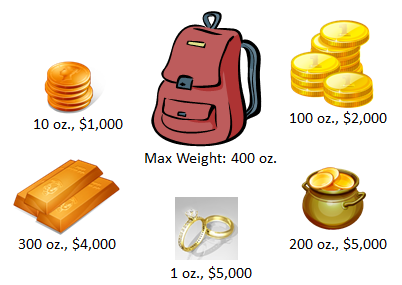
\includegraphics[scale=0.7]{./knapsack_problem.png}
	\caption{Ποιά είναι η καλύτερη επιλογή αντικειμένων;}
\end{figure}

Θα αναφερθούμε εκτενώς στο \(\textbf{0-1 Knapsack problem}\)  ή αλλιώς \(\textbf{Binary Knapsack problem}\). \\

Σε αυτή την παραλλαγή της οικογένεια των Knapsack problems πρέπει από ένα σύνολο n αντικειμένων να επιλέξουμε ένα υποσύνολο αυτών, έτσι ώστε να μεγιστοποιηθεί το κέρδος από την επιλογή των αντικειμένων που κάναμε, χωρίς όμως να υπερβούμε την καθορισμένη χωρητικότητα C του σακιδίου. Κάθε αντικείμενο συμβολίζεται με j και έχει δύο χαρακτηριστικά, το βάρος του που στο εξής θα το συμβολίζουμε με \(w_{j}\) και την αξία του, που θα τη συμβολίζουμε με \(p_{j}\). \\

Συνεπώς, αν θέλουμε να αποδόσουμε τον παραπάνω ορισμό με μαθηματικά, αυτά έχουν ως εξής: \\

\begin{align*}
	n &: \text{πλήθος των αντικειμένων}  \\
	j  &: \text{το j-οστό αντικείμενο}  \\
 	p_{j} &: \text{η αξία του j-οστού αντικειμένου}  \\
 	w_{j} &: \text{το βάρος του j-οστού αντικειμένου}  \\
 	C &: \text{η χωρητικότητα του σακιδίου} \\
\end{align*} \\

\begin{align*}
	\max \sum_{j=1}^{n}{p_{j}x_{j}}
\end{align*}  
υπό τον περιορισμό:

\begin{align*}
	\sum_{j=1}^{n}{w_{j}x_{j}} \leq C
\end{align*}

όπου \(x_{j}\) είναι μία δυαδική μεταβλητή που δηλώνει αν έχουμε τοποθετήσει το \(j\)-οστό αντικείμενο στο σακίδιο.
 
 \[ x_{j} = 
 \begin{cases} 
 	1 & \text{αν το j-οστό αντικείμενο τοποθετηθεί στο σακίδιο} \\
 	0 & \text{αν το j-οστό αντικείμενο ΔΕΝ τοποθετηθεί στο σακίδιο}
 \end{cases}
 \]
\\ \\
Χβτγ κάνουμε τις εξής παραδοχές: \\
\begin{align*}
	\text{Τα } p_{j}, w_{j}, C \text{ είναι ακέραιοι αριθμοί.} \\
	 p_{j} \geq 0 \\
	 w_{j} \geq 0 \\
	 C \geq 0 \\
	 w_{j} \leq c \\
	 \sum_{j=1}^{n} w_{j} \geq C 
\end{align*}

\vspace{2in}

\pagebreak

\subsection*{2. Give a dynamic programming solution to the 0-1 knapsack problem.}

Μία αρχική προσέγγιση για την επίλυση του \(\textbf{0-1 Knapsack problem}\) είναι η bruteforce τεχνική. Κατσκευάζουμε όλους τους πιθανούς συνδυασμούς αντικειμένων και εξετάζουμε ποιος είναι ο καλύτερος, δηλαδή αυτός που μεγιστοποιεί το κέρδος, χωρίς όμως να παραβιάζει τη χωρητικότητα του σακιδίου. \\ \\

Οι συνδυασμοί αυτοί είναι \(2^{n}\) το πλήθος, αν έχουμε n αντικείμενα. Συνεπώς, η πολυπλοκότητα της bruteforce μεθόδου είναι O(\(n2^{n}\)). Άρα, η μέθοδος αυτή είναι "απαγορευτική". \\ \\

Μία εναλλακτική τεχνική για την επίλυση του 0-1 Knapsack problem είναι ο δυναμικός προγραμματισμός. \\ \\

Ο δυναμικός προγραμματισμός χρησιμοποιείται για την
επίλυση προβλημάτων βελτιστοποίησης. Πρόκειται για μία μέθοδο επίλυσης προβλημάτων μέσω του συνδυασμού των λύσεων κάποιων υποπροβημάτων. Εφαρμόζεται όταν τα διάφορα υποπροβλήματα επκαλύπτονται. Ο δυναμικός προγραμματισμός (σε αντίθεση με άλλες τεχνικές, όπως το "διαίρει και κυρίευε") επιλύει το κάθε υποπρόβλημα μόνο μία φορά και το αποθηκεύει σε ένα πίνακα, έτσι ώστε να μη χρειαστεί να υπολογίσει ξανά τη λύση του ίδιου υποπροβλήματος. \\ \\

Θεωρούμε το υποπρόβλημα 0-1 Knapsack που αποτελείται από τα αντικείμενα 1, 2, ..., m και τη χωρητικότητα c, όπου \(1 \leq m \leq n\) και \(0 \leq c \leq C\). Το πρόβλημα διασπάται σε n υποπροβλήματα. Το m αυξάνεται, παίρνοντας τιμές από το 1
έως το n και σε κάθε υποπρόβλημα m, υπολογίζεται η τιμή \(f_{m}(c)\) καθώς το
c μεγαλώνει από το 0 έως το C. \\ \\

Η βέλτιστη λύση για αυτό το στιγμιότυπο είναι: 
\begin{align*}
	f_{m}(c) = \max {\sum_{j=1}^{m}{p_{j}x_{j}}} \text{ όπου } \\
	\sum_{j=1}^{m}{w_{j}x_{j}} \leq c \\
	x_{j} = 1 \text{ ή } 1 \text{ για } j=1,2,...,m
\end{align*}

και ισχύει ότι

 \[ f_{m}(c) = 
\begin{cases} 
f_{m-1}(c) & \text{ για } c = 0,...,w_{m}-1 \\
\max \left( f_{m-1}(c), f_{m-1}(c-w_{m}) + p_{j} \right) & \text{ για } c = w_{m},...,C
\end{cases}
\]

Στη συνέχεια παραθέτουμε αλγόριθμο που επιλύει το 0-1 Knapsack: \\ \\

\(\textbf{Βήμα 1:}\) \\
Κατασκευάζουμε έναν πίνακα \((n+1) \times (c+1)\). Η γραμμή j υποδηλώνει ότι έχουμε στη διάθεσή μας μόνο αντικείμενα 1,...,j. Η στήλη i υποδηλώνει ότι έχουμε χωρητικότητα σακιδίου i. Συνεπώς, αν ονομάζουμε τον πίνακα Κ, τότε το Κ[j][i] στοιχείο του πίνακα είναι η μεγαλύτερη "αξία" που μπορούμε να αποκομίσουμε από τα αντικείμενα 1,...,j με σακίδιο χωρητικότητας i. \\
\(\textbf{Βήμα 2:}\) \\
Τοποθετούμε τις αρχικές τιμές στον πίνακα, που δε χρειάζονται ιδιαίτερη υπολογιστική διαδικασία. Τα κελιά του πίνακα που μπορούμε να συμπληρώσουμε αμέσως είναι η γραμμή 0, όπου αν δεν έχουμε κανένα αντικείμενο, θα έχουμε 0 τελική αξία και η στήλη 0, όπου αν το σακίδιο έχει μηδενική χωρητικότητα δε μπορούμε να αποθηκεύσουμε κανένα αντικείμενο. \\ 
\(\textbf{Βήμα 3:}\) \\
Υπολογίζουμε την τιμή για το κελι Κ[j][i], λαμβάνοντας υπόψη τα προηγούμενα κελιά. Υπάρχουν δύο εκδοχές, είτε να τοποθετήσουμε το αντικείμενο j στο σακίδιο, είτε όχι. Αν δεν τοποθετήσουμε το αντικείμενο στο σακίδιο, τότε η μέγιστη τιμή που μπορούμε να λάβουμε στη συγκεκριμένη περίπτωση βρίσκεται  στο Κ[j-1][i]. Αν επιλέξουμε να τοποθετήσουμε το αντικείμενο στο σακίδιο (αυτό σημαίνει ότι τα βάρος του είναι κατάλληλο σε σχέση με τη χωρητικότητα που έχει τη δεδομένη στιγμή το σακίδιο), τότε το κελί Κ[j][i] είναι ίσο με την αξία του αντικειμένου j συν τη μέγιστη αξία που έχει προκύψει από τα προηγούμενα αντικείμενα, που χωρούν να μπούν στο σακίδιο μετά την καταχώρηση του j-οστού αντικειμένου στο σακίδιο. Συμπληρώνουμε όλον τον πίνακα. (Σημείωση: θέλουμε να χρησιμοποιήσουμε όλη τη χωρητικότητα του σακιδίου ή έστω να κάνουμε όσο καλύτερη δυνατή εκμετάλλευση του χώρου του).  \\
\(\textbf{Βήμα 4:}\) \\
Η τελική απάντηση στο 0-1 Knapsack problem βρίσκεται στη θέση Κ[n+1][c+1].

\vspace{2in}

\pagebreak

\subsection*{3. Give real world applications of knapsack problem.}

Το knapsack problem (πρόβλημα του σακιδίου) έχει πολλές πρακτικές εφαρμογές. Συγκεκριμένα, εφαρμόζεται άμεσα  στα προβλήματα που συναντάμε στη ζωή, που σχετίζονται με "πηγές" που έχουν συγκεκριμένη "αξία" και επιθυμούμε να επιλέξουμε από αυτές, περιοριζοντας όσο το δυνατό καλύτερα το τελικό κόστος της επιλογής μας.\\

Στη συνέχεια θα αναφέρουμε μερικά τέτοια παραδείγματα: \\
\(\bullet\) Ως πρώτο παράδειγμα θα αναφέρουμε εκείνο, στο οποίο οφείλει και το όνομά του το knapsack problem. Η προετοιμασία της βαλίτσας για κάποιο ταξίδι. Η βαλίτσα έχει συγκεκριμένο διαθέσιμο χώρο για να φιλοξενήσει τα πράγματά μας. Πρέπει να γίνει η καλύτερη επιλογή αντικειμένων (ρούχα, προσωπικά αντικείμενα κτλ.), ώστε να υπάρχουν όλα τα απαραίτητα μέσα στη βαλίτσα (κι αν ταξιδεύουμε με αεροπλάνο, το βάρος όλων των αντικειμένων να μην υπερβαίνει κάποιο ορισμένο όριο κιλών). \\

\(\bullet\) Η αποθήκευση εμπορευμάτων σε αποθήκες. Ο χώρος της αποθήκης είναι καθορισμένος και δεν μεταβάλλεται και πρέπει σε αυτόν το χώρο να μπορέσουν να χωρέσουν όσο το δυνατό περισσότερα εμπορεύματα. Απλουστεύοντας τα δεδομένα, μπορόυμε να υποθέσουμε ότι περισσότερα προϊόντα στην αποθήκη, σημαίνει αύξηση των κερδών της επιχείρησης. \\

\(\bullet\) Οι κατάλληλες επενδύσεις. Έστω  ότι επιθυμούμε να επενδύσουμε όλα ή ένα  μέρος  από τα κεφάλαια. Έχουμε να επιλέξουμε ανάμεσα  σε κάποιες πιθανές επενδύσεις. Κάθε επένδυση έχει ένα συγκεκριμένο κόστος και ένα αναμενόμενο κέρδος. Η βέλτιστη επιλογή μπορεί να βρεθεί με το πρόβλημα του σακιδίου. \\ 

\(\bullet\) Η επιλογή υπαλλήλων για μία επιχείρηση. Υπάρχουν πολλοί εν δυνάμει υπάλληλοι, με διαφορετικές ικανότητες, ταλέντα, γνώσεις, πτυχία και πιστοποιήσεις, αλλά ταυτόχρονα και με διαφορετικές μισθολογικές απαιτήσεις. Η επιχείρηση είναι σε θέση να διαθέτει ένας συγκεκριμένο ποσό για μισθοδοσίες και μπορεί να παρέχει καθορισμένες παροχές στους εργαζομένους της (π.χ. κτηριακές υποδομές). Ποιά είναι η καλύτερη επιλογή εργαζομένων, ώστε η επιχείρηση να αυξήσει τα κέρδη της; \\

\(\bullet\) Στο σημείο αυτό θα αναφερθούμε σε ένα πραγματικό παράδειγμα εφαρμογής του προβλήματος του σακιδίου. Η εταιρεία Trashy Bags είναι μία εταιρεία ευαισθητοποιημένη στο θέμα των πλαστικών απορριμάτων, που είναι ένα θέμα ζωτικής σημασίας για τον πλανήτη. Επιλέγει να ανακυκλώνει και να επαναχρησιμοποιεί το πλαστικό. Μία ομάδα συλλεκτών συλλέγει από τους δρόμους γύρω στα 15 εκατομμύρια πλαστικές σακούλες. Τελικά, από το πλαστικό που έχει συλλέξει κατασκευάζει τσάντες και αδιάβροχα. Άρα, στην περίπτωση αυτή, η εταιρεία επιθυμεί να αυξήση την παραγωγή της, επιλέγοντας τα καλύτερα (πλαστικά) αντικείμενα, με σκοπό να παραχθεί ο απαιτούμενος  αριθμός  παραγόμενων προϊόντων και τελικά η εταιρεία να αυξήσει τα κέρδη της. Ο περιορισμός εδώ σχετίζεται με το κόστος που προκύπτει από το κόστος συλλογής απορριμμάτων από πλαστικές σακούλες,  το  κόστος  επεξεργασίας  και  το  κόστος  πώλησης  των προϊόντων. \\

\(\bullet\) Η επιλογή διαφημίσεων σε κάποιο ραδιοφωνικό/τηλεοπτικό σταθμό. Υπάρχει συγκεκριμένο πλήθος διαφημίσεων. Κάθε διαφήμιση έχει μία τιμή και κάποιον χρόνο. Στόχος είναι να μεταδοθούν όσο το δυνατό περισσότερες κερδοφόρες διαφημίσεις, χωρίς όμως να ξεπεραστεί ένα προκαθορισμένο χρονικό όριο. \\

\begin{figure}[!]
	\centering
	
\includegraphics[scale=0.65]{./knapsack-example.png}
	\caption{Μόνο με χιουμοριστική διάθεση..}
\end{figure}




\pagebreak

\subsection*{4. Define the Subset sum problem and give a dynamic programming solution for
	it. Write down the difference between the subset sum and the knapsack problem.}

Το \(\textbf{Subset sum problem}\) είναι ένα πρόβλημα απόφασης στην υπολογιτική.... και την κρυπτογραφία. Υπάρχουν πολλές εκδοχές για αυτό το πρόβλημα. Το Subset sum problem αναζητά το υποσύνολο από ένα σύνολο ακεραίων αριθμών, το οποίο αν αθροίσουμε τους αριθμούς του, το αποτέλεσμα που θα προκύψει να είναι 0. Το πρόβλημα αυτο NP-complete. Είναι εύκολο αν κάποιος μας δώσει την απάντηση σε ένα τέτοιο πρόβλημα να αποφανθούμε αν είναι valid ή όχι, αλλά είναι δύσκολο να τη βρούμε μόνοι μας. \\ \\

Το Subset sum problem ή αλλιώς Value Independent Knapsack Problem ή Stickstacking Problem μπορεί να θεωρηθεί στιγμιότυπο του 0-1 Knapsack problem. Πρέπει να επιλέξουμε ένα υποσύνολο βαρών, τέτοιο ώστε το άθροισμά τους να είναι το μεγαλύτερο δυνατό και ταυτόχρονα να μην υπερβαίνει τη χωρητικότητα του σακιδίου. \\ \\

Έστω ότι έχουμε n αντικείμενα συνολικά και ένα σακίδιο χωρητικότητας C. Κάθε αντικείμενο j έχει βάρος \(w_{j}\). Στόχος είναι να επιλεγεί ένα υποσύνολο αντικειμένων τέτοιο ώστε το συνολικό βάρος τους να είναι ίσο ή να μη ξεπερνά τη χωρητικότητα του σακιδίου. \\ \\ 

Η μαθηματική μοντελοποίηση όσων αναφέραμε είναι: \\

\begin{align*}
	\max \sum_{j=1}^{n}{w_{j}x_{j}}
\end{align*} 

υπό τον περιορισμό:

\begin{align*}
	\sum_{j=1}^{n}{w_{j}x_{j}} \leq C
\end{align*}

με 

 \[ x_{j} = 
\begin{cases} 
1 & \text{αν το j-οστό αντικείμενο τοποθετηθεί στο σακίδιο} \\
0 & \text{αν το j-οστό αντικείμενο ΔΕΝ τοποθετηθεί στο σακίδιο}
\end{cases}
\]

Χβτγ ισχύει ότι: \\
\begin{align*}
\text{Τα } w_{j}, C \text{ είναι ακέραιοι αριθμοί.} \\
w_{j} \geq 0 \\
C \geq 0 \\
w_{j} \leq c \\
\sum_{j=1}^{n} w_{j} \geq C 
\end{align*}

Ουσιαστικά, το Subset sum problem είναι ειδική περίπτωση του 0-1 Knapsack problem. Το 0-1 Knapsack problem γίνεται Subset sum problem αν η "αξία" στην περίπτωση του 0-1 Knapsack problem είναι ταυτόσημη με το βάρος του  του j-οστού αντικειμένου, \(p_{j} = w_{j}, \forall j\). \\ \\

To Subset sum problem μπορεί να επιλυθεί με χρήση Δυναμικού προγραμματισμού, καθώς είναι "στιγμιότυπο" του 0-1 Knapsack problem. Παραθέτουμε ένα ειδικά σχεδιασμένο αλγόριθμο για αυτήν την παραλλαγή της Knapsack οικογένειας προβλημάτων.\\ \\

\(\textbf{Βήμα 1:}\) \\
Κατασκευάζουμε έναν πίνακα \((n+1) \times (c+1)\), στον οποίο καταχωρίζουμε true ή false. Η γραμμή j υποδηλώνει ότι έχουμε στη διάθεσή μας μόνο τους αριθμούς 1,...,j. Η στήλη i υποδηλώνει ότι θέλουμε να επιτύχουμε άθροισμα i. Συνεπώς, αν ονομάζουμε τον πίνακα Κ, τότε το Κ[j][i] στοιχείο του πίνακα δηλώνει αν μπορούμε ή όχι να επιτύχουμε άθροισμα ίσο με i, με διαθέσιμους προσθεταίoυς τους αριθμους 1,...,j. \\
\(\textbf{Βήμα 2:}\) \\
Τοποθετούμε τις αρχικές τιμές στον πίνακα, που δε χρειάζονται ιδιαίτερη υπολογιστική διαδικασία. Τα κελιά του πίνακα που μπορούμε να συμπληρώσουμε αμέσως είναι εκείνα της γραμμής 0,με false, καθώς αν δεν έχουμε κανέναν διαθέσιμο αριθμό, δε μπορούμε να επιτύχουμε άθροισμα και της στήλης 0, με true, αφού το άθροισμα του κενού υποσυνόλου είναι 0. \\ 
\(\textbf{Βήμα 3:}\) \\
Υπολογίζουμε την τιμή για το κελι Κ[j][i], λαμβάνοντας υπόψη τα προηγούμενα κελιά. Υπάρχουν δύο εκδοχές, είτε να τοποθετήσουμε στο υποσύνολο των προσθεταίων τον αριθμό j, είτε όχι. Αν υπάρχει υποσύνολο ακεραίων από το 1 ως το j-1, τέτοιο ώστε \(\sum_{k=1}^{j-1}k = i\), τότε στο κελί Κ[j][i] τοποθετούμε true, αλλιώς τοποθετούμε false. \\ 
\(\textbf{Βήμα 4:}\) \\
Η τελική απάντηση στο Subset sum problem βρίσκεται στη θέση Κ[n+1][c+1].

\vspace{2in}

\pagebreak

\subsection*{References:}

1. "Εισαγωγή στους αλγορίθμους", Thomas H. Cormen, Charles E. Leiserson, Ronald L. Rivest, Clifford Stein, Πανεπιστημιακές εκδόσεις Κρήτης, ISBN: 978-960-524-473-6 \\ \\

2. "KNAPSACK PROBLEM", Αθανασοπούλου Δήμητρα, Πανεπιστήμιο Πατρών, Διατμηματικό Πρόγραμμα Μεταπτυχιακών Σπουδών Μαθηματικά των Υπολογιστών και των Αποφάσεων, Διπλωματική εργασία, 2017. \\ \\

3. "How to solve the Knapsack Problem with dynamic programming",  https://medium.com/@fabianterh/how-to-solve-the-knapsack-problem-with-dynamic-programming-eb88c706d3cf \\ \\

4. "Subset sum problem", https://en.wikipedia.org/wiki/Subset\_sum\_problem \\ \\ 

5. "Subset Sum Problem using Dynamic Programming (O(N*sum) time complexity)", https://iq.opengenus.org/subset-sum-problem-dynamic-programming/ \\ \\

\end{document}
